\chapter{TRIGGER SYSTEM}
\label{chap:Trigger}
%%%%%%%%%%%%%%%%%%%%%%%%%%%%%%%%%%%%%%%%%%%%%%%%%%%%%%%
%%%%%%%%%%%%%%%%%%%%%%%%%%%%%%%%%%%%%%%%%%%%%%%%%%%%%%%
%%%%%%%%%%%%%%%%%%%%%%%%%%%%%%%%%%%%%%%%%%%%%%%%%%%%%%%

\section{Overview of the CMS trigger}
\label{sec:trigOverview}
Many more collisions occur within the LHC than can be stored and analyzed. At the four interaction points of the LHC, bunches of protons collide every 25 ns. For every bunch crossing, there are on average 25 ``soft-scatter" collisions (pileup). This corresponds to an overall event rate of 1 GHz. Given that each event produces approximately 1 MB of data, it is impossible to store every event or even the majority of events. This has been especially true in recent years, with the LHC continually breaking new records for instantaneous luminosity. 

To solve this problem, the CMS detector includes a sophisticated trigger system to determine which events get written to tape and eventually analyzed. The CMS trigger  is divided into two steps: the hardware-based Level 1 (L1) trigger, and the software-based High Level Trigger (HLT). The L1 trigger reduces the rate from 1 GHz to approximately 100 kHz, and the HLT makes the final decisions necessary to reduce the rate to a few hundred Hz, the maximum amount that can be written and stored. The L1 trigger and the HLT are both highly configurable, which allows CMS to define and alter the thresholds as needed to suit different running conditions. Both steps of the CMS trigger are described in more detail below. 

%%%%%%%%%%%%%%%%%%%%%%%%%%%%%%%%%%%%%%%%%%%%%%%%%%%%%%%
%%%%%%%%%%%%%%%%%%%%%%%%%%%%%%%%%%%%%%%%%%%%%%%%%%%%%%%

\section{Level 1 trigger}
\label{sec:L1}
The L1 trigger performs rough calculations of event parameters using field-pro-grammable gate arrays located in the detector cavern. The L1 trigger only has 3.8 $\mu$s to make a decision about each event in order to reduce the output event rate to 100 kHz \cite{L1trig}. For inputs, the L1 trigger receives data from the ECAL, HCAL, and muon detector subsystems. The L1 trigger is naturally divided into two paths. The calorimeter trigger, shown schematically in Figure~\ref{fig:caloL1T}, takes data from the ECAL and HCAL subsystems and builds photon, electron, and jet candidates, as well as overall event quantities such as missing transverse momentum and total hadronic activity. The second half of the L1 trigger is the muon trigger, and its overall structure is shown in Figure~\ref{fig:muonL1T}. The output from the muon and calorimeter triggers goes into the Global Trigger (GT) processor \cite{L1_GT}, which makes the final decision regarding whether or not to accept the event. 

%%%%%%%%%%%%%%%%%%%%%%%%%%%%%%%%%%%%%%%%%%%%%%%%%%%%%%%

\subsection{Calorimeter trigger}
As shown in Figure~\ref{fig:caloL1T}, the raw inputs for the calorimeter trigger are trigger primitives (TP) from the ECAL and the HCAL. The trigger primitives from the HCAL are divided between the HCAL Barrel and Endcap (HB and HE, respectively), and the forward HCAL (HF). Trigger primitives consist of coarse information about the energy deposits  in the calorimeter for every bunch crossing. The ECAL is divided into trigger towers, groups of crystals corresponding to a region of approximately 0.087 $\times$ 0.087 in $\eta$ and $\phi$, and a TP is generated by summing the energy from each crystal in the tower. In the HCAL, TPs are generated for each trigger tower by summing the transverse energy in two consecutive time slices. 

Layer-1 of the calorimeter trigger collects the TPs from the ECAL and HCAL. Its primary role is to distribute the data to one of nine Layer-2 nodes. Each Layer-2 node receives the full set of of TPs for a particular bunch crossing, and identifies photon, electron, jet, and $\tau$-tagged jet candidates using several dynamic clustering and local maxima finding algorithms. The outputs from the Layer-2 nodes are fed into a de-multiplexing (demux) node, which ranks the candidates by transverse momentum and sends the data to the Global Trigger. 

%CITE http://iopscience.iop.org/article/10.1088/1748-0221/12/03/C03021/pdf
%CITE http://iopscience.iop.org/article/10.1088/1748-0221/11/02/C02029/pdf
%Maybe also https://arxiv.org/pdf/1609.02366.pdf

\begin{figure*}[h]
\begin{center}
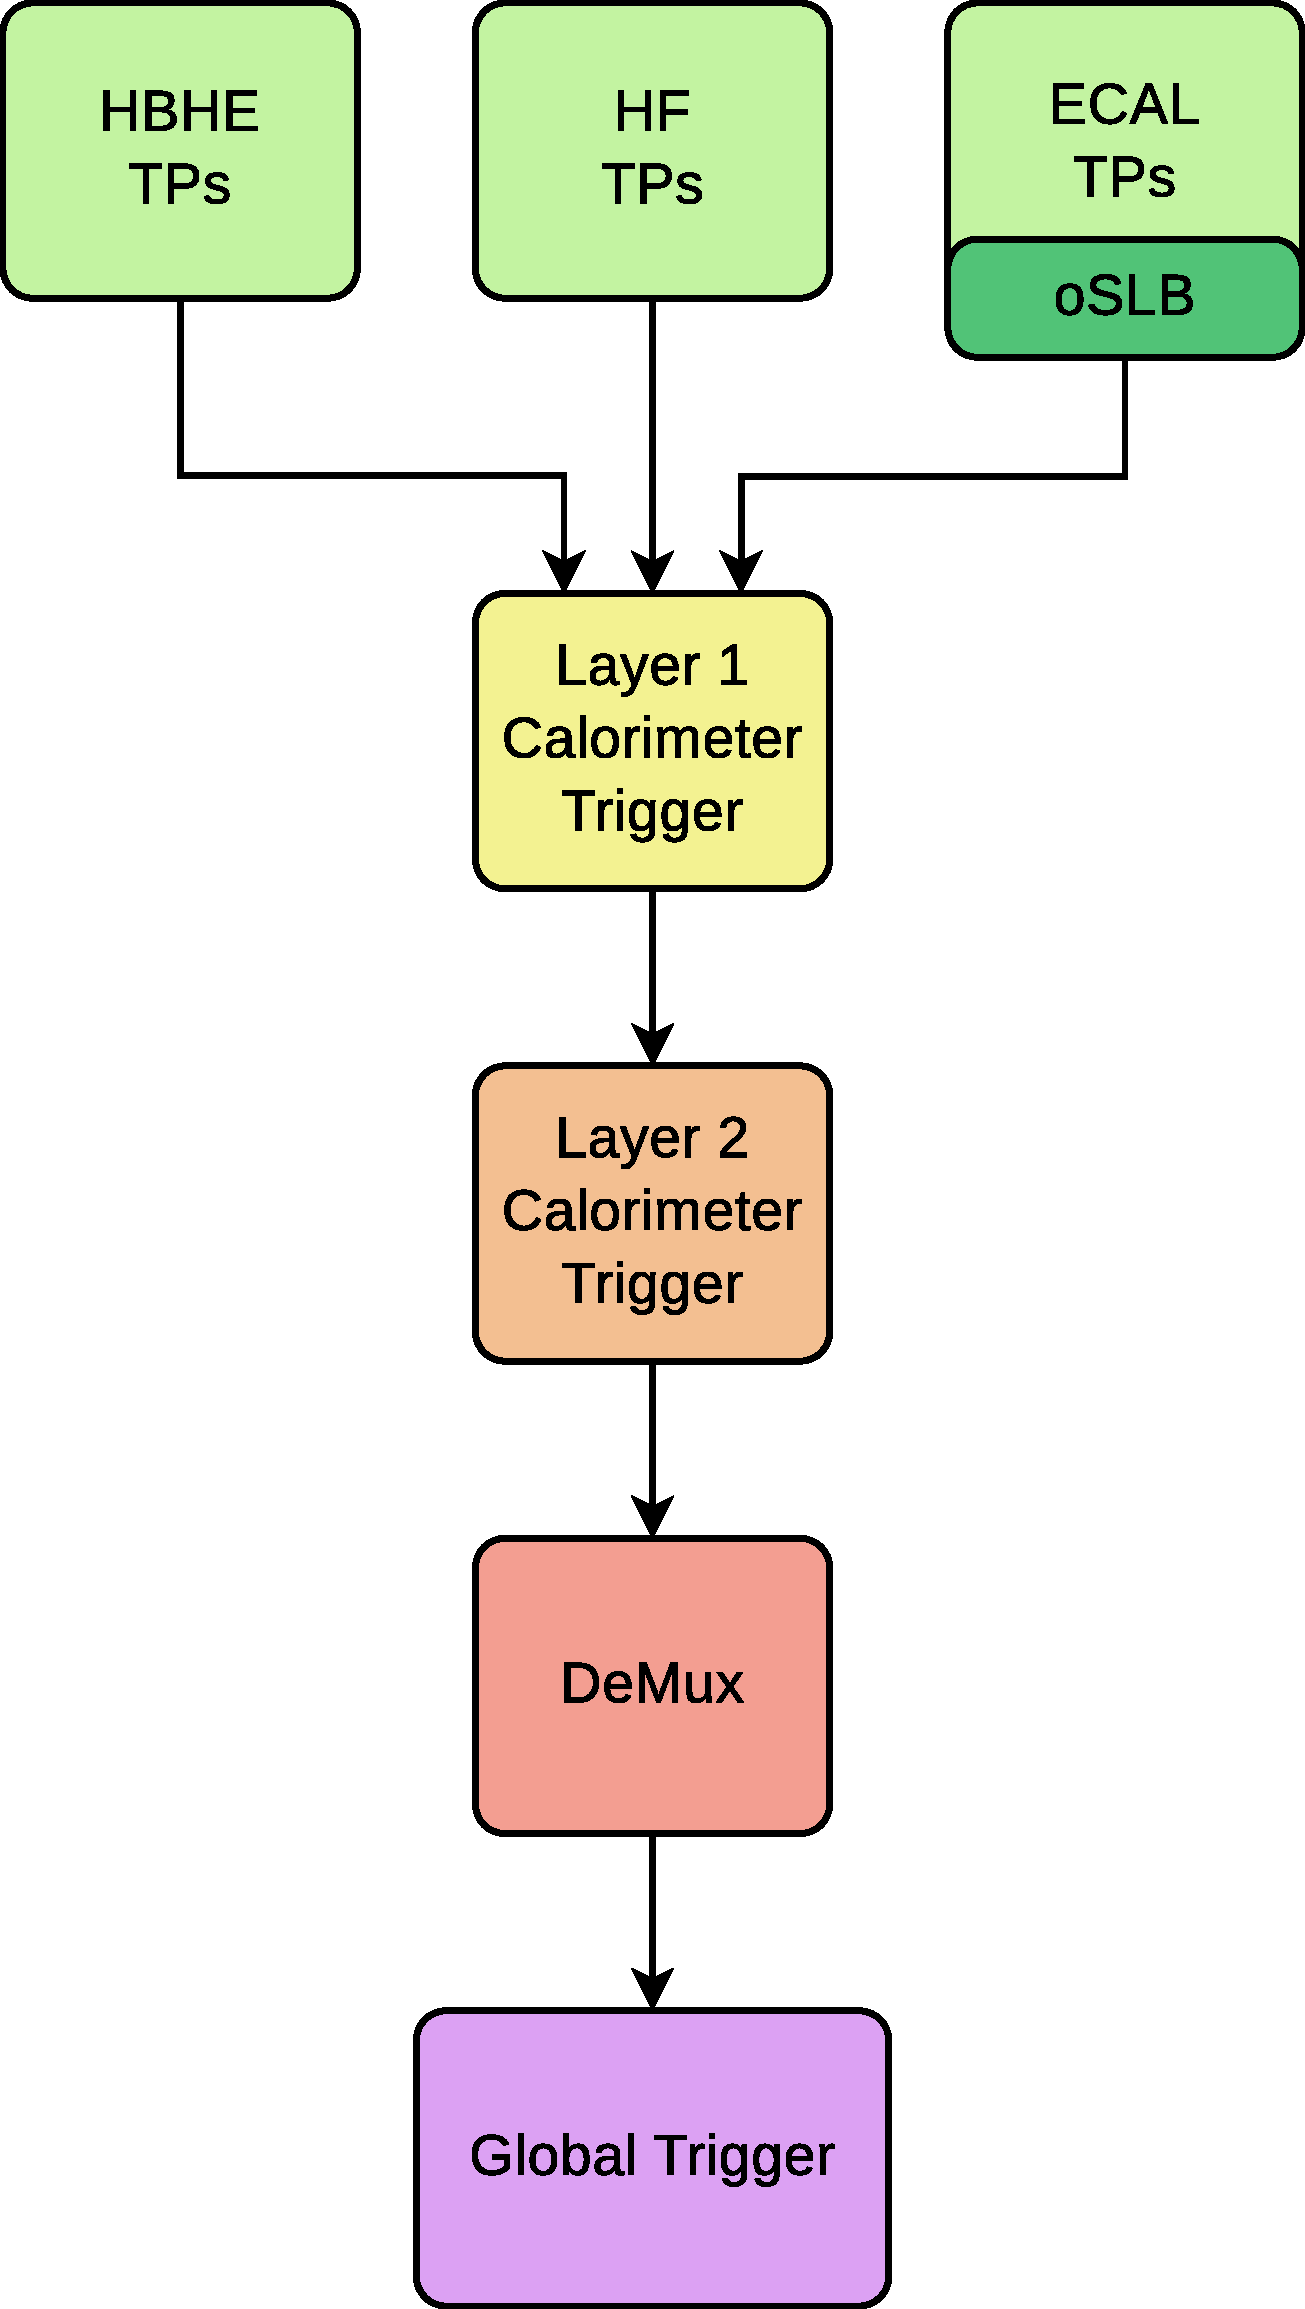
\includegraphics[width=0.6\textwidth]{Figures/Trigger/caloL1T.pdf}
\end{center}
\caption{Schematic showing the overall structure of the calorimeter half of the L1 trigger. Reprinted from Reference~\cite{L1twiki}.}
\label{fig:caloL1T}
\end{figure*}

%%%%%%%%%%%%%%%%%%%%%%%%%%%%%%%%%%%%%%%%%%%%%%%%%%%%%%%

\subsection{Muon trigger}
Information from all three of the muon detector subsystems---the cathode strip chamber (CSC) detectors, resistive plate chamber (RPC) detectors, and drift tubes (DT)---are combined in the L1 muon trigger to reconstruct muon candidates and their momenta. The muon trigger has three track-finding subsystems that reconstruct muons for different $|\eta|$ regions: the barrel track finder ($|\eta| < 0.83$), the endcap track finder ($|\eta| > 1.24$), and the overlap track finder ($0.83 < |\eta| < 1.24$).

Trigger primitives from the DT and RPC detectors are first combined in the TwinMUX system into ``super-primitives". This step serves to increase the precision of the position and timing of muon hits by taking advantage of the redundancy between the two subsystems.  The barrel track finder uses the super-primitives as inputs for its track finding algorithm, processing twelve 30$^{\circ}$ wedges in parallel. 

The endcap track finder receives information from the CSC detectors, and the overlap track finder uses information from all three subsystems. Both of these track finders use large look-up tables to convert specific hit patterns into \pT assignments for the muon candidates.

The outputs from all three track finders are sent to the Global Muon Trigger, which ranks the muons by quality and transverse momentum and sends the top 8 muon candidates to the Global Trigger for a final decision on the event.

\begin{figure*}[h]
\begin{center}
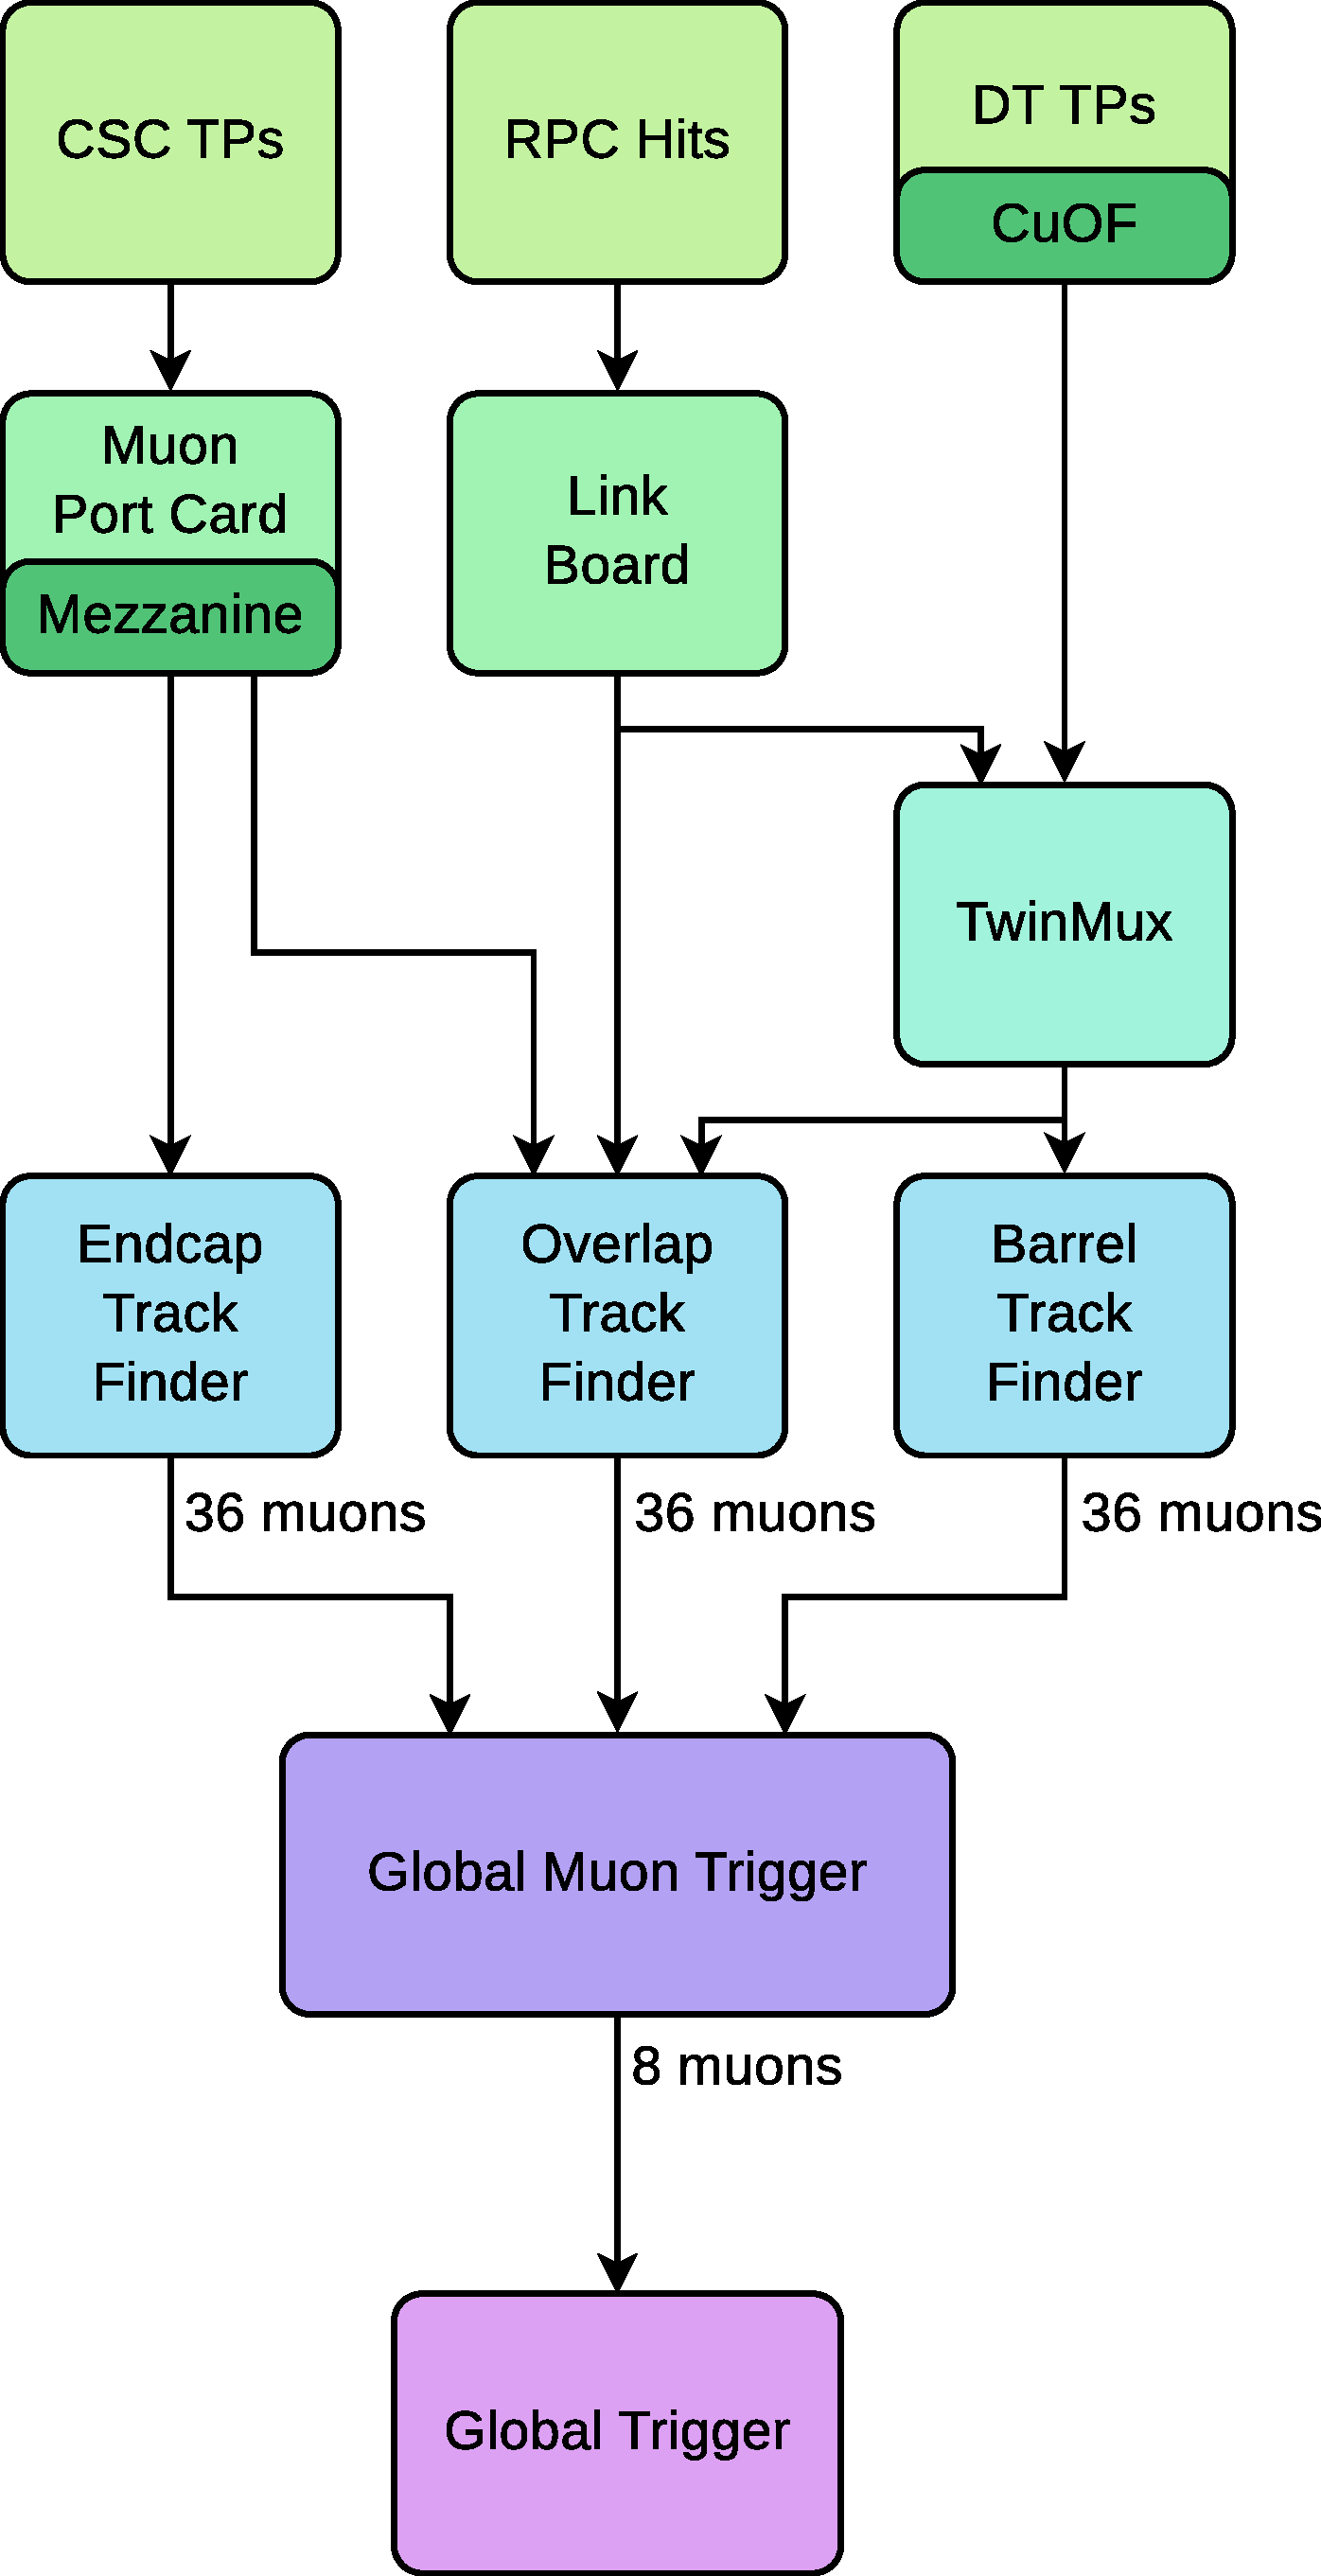
\includegraphics[width=0.7\textwidth]{Figures/Trigger/muonL1T.pdf}
\end{center}
\caption{Schematic showing the overall structure of the muon half of the L1 trigger. Reprinted from Reference~\cite{L1twiki}.}
\label{fig:muonL1T}
\end{figure*}

\subsection{Global Trigger}
The reconstructed objects and quantities built by the calorimeter trigger and the muon trigger---photon, electron, jet, and muon candidates, missing energy and total hadronic activity---get sent to the Global Trigger (GT) for final processing. The GT can implement up to 512 different trigger algorithms using these objects \cite{L1_GT}. For example, one of the L1 algorithms (or ``seeds") used in this analysis is DoubleEG\_22\_12.  This path requires two electron or photon candidates with leading and trailing \pT greater than 22 and 12 GeV, respectively.

A full set of L1 algorithms is known as the L1 menu. The menu can be adjusted as needed to meet the requirements of the CMS physics program. 
In particular, the ``prescale" of each L1 seed can be adjusted 
to take full advantage of varying LHC running conditions and instantaneous luminosities. 
A prescale is an integer value $N$ used to reduce the rate of a trigger path by only applying the trigger to
1 out of every $N$ events. For the 2016 data-taking period, the lowest unprescaled DoubleEG seed was
DoubleEG\_22\_12, but the menu also included several prescaled algorithms with lower \pT thresholds.

%%%%%%%%%%%%%%%%%%%%%%%%%%%%%%%%%%%%%%%%%%%%%%%%%%%%%%%
%%%%%%%%%%%%%%%%%%%%%%%%%%%%%%%%%%%%%%%%%%%%%%%%%%%%%%%

\section{High Level Trigger}
\label{HLT}
The High Level Trigger (HLT) uses a large farm of commercially available PCs to further reduce the rate to a few hundred Hz. The HLT receives fully-built event data from the CMS data acquisition system (DAQ) and processes only those bunch crossings that have passed the L1 trigger. The 13,000 CPU cores used in the HLT run the CMS software framework referred to as CMSSW, the same framework that is used in the offline analysis. 

Approximately 400 HLT ``paths" are used to select events of interest. Each HLT path is a single set of criteria for accepting an event if it satisfies a particular physics signature. The full list of HLT paths is referred to as the HLT menu. The HLT menu is often updated to reflect improvements in the software, updates to the calibrations, changes to the beam condition, or revisions to the physics signatures being sought. 

The HLT has a limited amount of time it can spend making a decision on a single bunch crossing. For this reason, each HLT path is ``seeded" by one or more L1 algorithms. When an event gets passed to the HLT from the DAQ, the HLT only processes those paths that are seeded by L1 bits that fired. 
For example, the diphoton HLT path used in this analysis is seeded by a combination of single and double e/$\gamma$ (EG) L1 algorithms. If none of those particular L1 seeds fired, then the HLT path will not get run on that event. 

In addition, significant time is saved at the HLT by running the steps (filters) of each HLT path in order from least CPU intensive to most CPU intensive. If the event fails any of the filters in an HLT path, then the processing is immediately aborted and the remaining filters do not get run. In the diphoton HLT path described below, the most CPU intensive filter is the invariant mass calculation, and therefore it runs only if the event has already satisfied the rest of the path's requirements.

Based on its general physics signature, each HLT path is assigned to a primary data set (PD). For this analysis, signal events are included in the DoubleEG PD. The SingleElectron and SinglePhoton data sets are also used for object identification studies.

%%%%%%%%%%%%%%%%%%%%%%%%%%%%%%%%%%%%%%%%%%%%%%%%%%%%%%%
%%%%%%%%%%%%%%%%%%%%%%%%%%%%%%%%%%%%%%%%%%%%%%%%%%%%%%%
%%%%%%%%%%%%%%%%%%%%%%%%%%%%%%%%%%%%%%%%%%%%%%%%%%%%%%%

\section{Analysis triggers}
\label{sec:analysisTrig}

The HLT paths used in this analysis are listed in Table~\ref{tab:triggers}. These triggers were developed for the $H \rightarrow \gamma\gamma$ search, 
but also serve our analysis well. Two triggers are used: a primary trigger that requires the diphoton invariant mass to be greater than 90 GeV, and a control
trigger that was designed to collect $Z\rightarrow ee$ events. 

\begin{table}[ht]
\caption{HLT TRIGGER PATHS}
\label{tab:triggers}
\begin{center}
\begin{tabular}{|c|}
\hline
\hline
\bf{Primary Trigger}   \\                                                                                                 
HLT\_Diphoton30\_18\_R9Id\_OR\_IsoCaloId\_AND\_HE\_R9Id\_Mass90\_v* \\     
\hline                                               
\bf{Control Sample Trigger} \\                                                                                       
HLT\_Diphoton30\_18\_R9Id\_OR\_IsoCaloId\_AND\_HE\_R9Id\_ \\
DoublePixelSeedMatch\_Mass70\_v* \\                              
\hline
\hline
\end{tabular}
 \justify{List of triggers used to accumulate the events in the 35.9~\fbinv data sample.}
\end{center}
\end{table}

\subsection{Trigger requirements}
\label{sec:trigRequirements}
The requirements to pass the various parts of the trigger
are listed in Table~\ref{tab:trigcuts}.
Because we only use photons with $|\eta| < 1.4442$ in this analysis
(see Chapter~\ref{chap:EventSelect} for full event selection requirements), we list only
the trigger requirements in the barrel. 

\begin{table}[ht]
\caption{PRIMARY TRIGGER REQUIREMENTS}
\label{tab:trigcuts}
\begin{center}
\begin{tabular}{|c| c |}
\hline
\hline
\textbf{Name} & \textbf{Cuts} \\
\hline
Diphoton30\_18\_ &  Leading photon \pt$ > 30$ GeV \\
 & Sub-leading photon \pt$ > 18$ GeV \\
 \hline
R9Id\_ & $R_9 > 0.85$\\
\hline
IsoCaloId\_ &  \sigmaietaieta$< 0.015$\\
 & ECAL isolation~$<~(6 + 0.012 \times$Photon \ET) \\
 & Track isolation~$<~(6 + 0.002 \times$Photon \ET) \\
 \hline
HE\_R9Id\_ & H/E $< 0.1$ \\
 & $R_9 > 0.5$\\
 \hline
Mass90\_  & $m_{\gamma\gamma} > 90$ GeV \\                                                                        
\hline
\hline
\end{tabular}
 \justify{Definition of cuts used in the primary analysis trigger, HLT\_Diphoton30\_18\_ R9Id\_OR\_IsoCaloId\_AND\_HE\_R9Id\_Mass90\_v*}
\end{center}
\end{table}

Each of the variables used in the trigger are defined below. See Chapter~\ref{chap:EventSelect} for more information on how energy deposits in the calorimeter are reconstructed into photon ``superclusters".

\begin{itemize}
\item{\ET:} The transverse energy \ET of a photon is defined
as the magnitude of the projection
of the photon momentum on the plane perpendicular to the beam axis.
\item{$R_9$:} The variable $R_9$ is
a measure of the overall transverse spread of the shower. It is the ratio
of the energy deposited in the ECAL inside a 3x3 crystal matrix centered on
the most energetic crystal in the supercluster to the supercluster
 raw energy.
\item{$\sigma_{i\eta i \eta}:$} The shower width \sigmaietaieta is
      the log-fractional energy-weighted spread within the 5x5 crystal matrix centered on the
      crystal with the largest energy deposit in the supercluster. The symbol
      i$\eta$ indicates that the variable is obtained by measuring position by
      counting crystals.
\item{ECAL isolation:} The ECAL isolation is
      the sum of all energy deposits in the ECAL within a cone of \dR
      $<$0.3 centered on the photon.
\item{Track isolation:} The track isolation is
      the sum of the energies of tracks in the tracker within a cone of \dR
      $<$0.3 centered on the photon.
\item{H/E:} The ratio between the energy deposited in the HCAL
      tower closest to the supercluster position and the energy deposited to
      that supercluster in the ECAL is referred to as H/E.
  \end{itemize}

All photons are required to pass the H/E and loose $R_9$ cuts in
\_HE\_R9Id\_, and either the tighter $R_9$ cuts in
\_R9Id\_ or the isolation and shape cuts in \_IsoCaloId\_.
The leading leg of the filter requires the photon candidate
to be matched to an L1 seed. It can be matched to one of several
SingleEG and DoubleEG L1 filters, but the largest contribution comes
from the lowest unprescaled triggers: namely, SingleEG40 and
DoubleEG$\_$22$\_$15.
Both photons must satisfy the trailing filter, which is unseeded.
In addition to the cuts listed above, the invariant mass of
the diphoton system is required to be greater than 90 GeV.

The control trigger shares all of the same requirements as the primary trigger, with two exceptions: 
the invariant mass of the two electromagnetic objects is required to be greater than 55 GeV rather than 90 GeV, 
and both electromagnetic objects are required to be matched to a pixel seed. A pixel seed is defined
as at least two hits in the pixel detectors that are consistent with the location of the energy deposit in the ECAL. 

%%%%%%%%%%%%%%%%%%%%%%%%%%%%%%%%%%%%%%%%%%%%%%%%%%%%%%%
%%%%%%%%%%%%%%%%%%%%%%%%%%%%%%%%%%%%%%%%%%%%%%%%%%%%%%%
%%%%%%%%%%%%%%%%%%%%%%%%%%%%%%%%%%%%%%%%%%%%%%%%%%%%%%%

\section{Trigger efficiency}
\label{sec:trigEff}
An important input to the analysis is the overall trigger efficiency. Due to the similarity of the ECAL response 
to electrons and photons, the trigger efficiency can be calculated from 
$Z\rightarrow ee$ events in data using the tag-and-probe method. In this method, two electron candidates
are required. One serves as the ``tag" and is required to pass loose photon identification criteria. 
The second electron candidate serves
as the ``probe" and has to satisfy the same selection criteria as our offline photon identification (see Section~\ref{sec:ObjSelect}). 
In order to ensure a high purity of electromagnetic objects, the invariant mass of the di-electron system must be between 75 and 105~GeV. 
For this study, tag-and-probe events were collected by requiring that the tag pass
a single electron control trigger, HLT\_Ele27\_WPTight\_Gsf.


The efficiency $\epsilon$ of the HLT path or trigger filter that is being studied is given by the following equation, where $N_{total}$ is the total number of tag and probe pairs 
passing all requirements, and $N_{pass}$ is the number of tag and probe pairs in which  the probe passes the trigger filter.
\begin{equation}
 \epsilon_{trig} = N_{pass} / N_{total}
\end{equation}

\subsection{Efficiency of primary trigger}
\label{sec:TnP_Eff}

Because our analysis trigger is seeded by the OR of multiple SingleEG and DoubleEG L1 seeds, the names of which changed over the course of the 2016 data-taking period, calculating the L1 efficiency on its own proved to be tricky. Instead, it was simpler to calculate the total efficiency with which photon candidates pass both the L1 seed and the leading leg of the HLT path. This efficiency as a function of photon \pt is shown in Figure~\ref{fig:leadEff}. The efficiency was fit to an error function to calculate the overall efficiency at the plateau. For photon \pt $>~40$ GeV, the leading filter is 98.2\% efficient.

\begin{figure*}[h]
\begin{center}
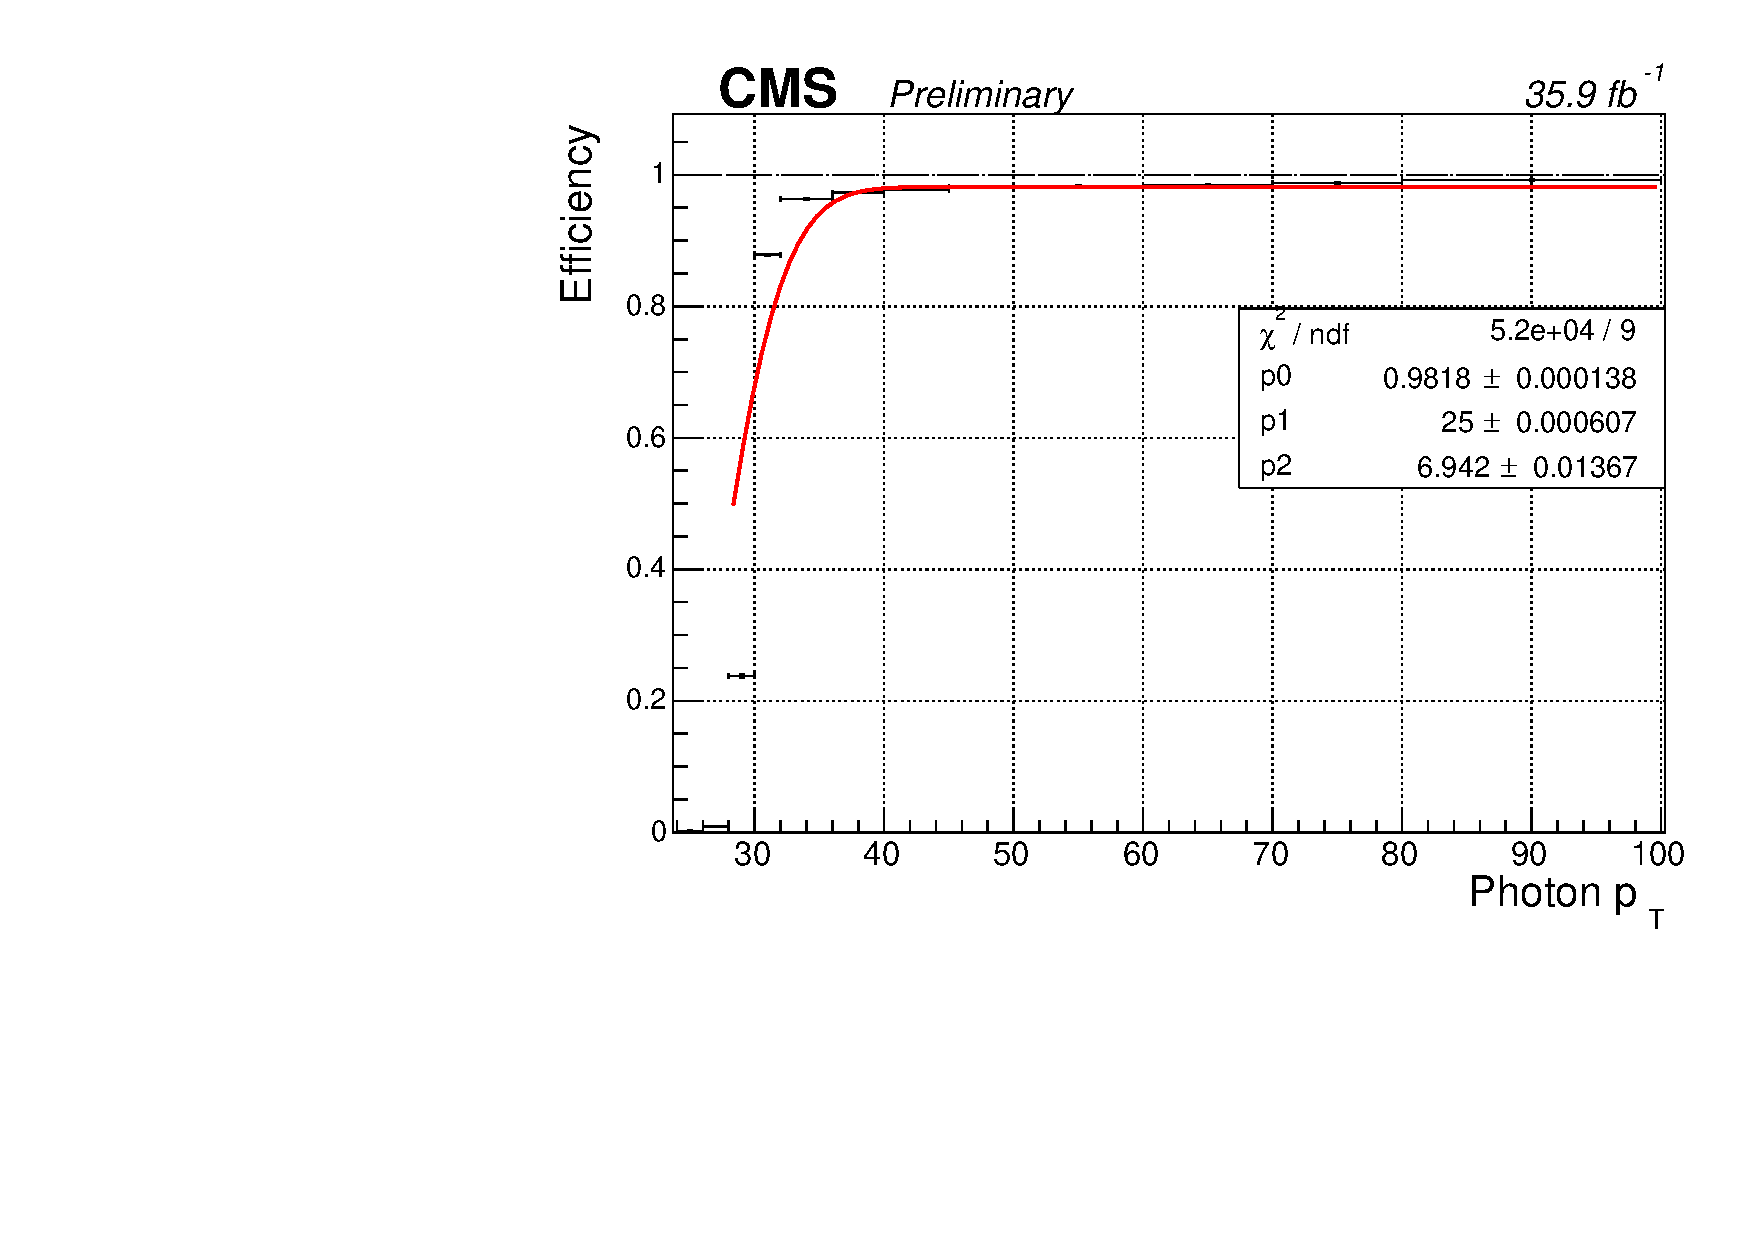
\includegraphics[width=0.9\textwidth]{Figures/Trigger/leadingEff.pdf}
\end{center}
\caption{Efficiency of the L1 seed and the leading leg of the primary analysis trigger with respect to photon \pT. 
For $\pT > 40$ GeV, the trigger is 98.2\% efficient.}
\label{fig:leadEff}
\end{figure*}

Tag and probe objects for the trailing leg efficiency must pass the same set of requirements as those used in the leading leg efficiency calculation, with the additional requirement that the tag must pass the leading filter. This requirement arises from the way HLT modules are structured. Filters are processed sequentially, and if an event fails one filter, the subsequent filters are skipped. Figure~\ref{fig:trailEff} shows the efficiency of the trailing filter as a function of photon \pt. For $\pT > 40$ GeV, the trigger is 99.8\% efficient.

\begin{figure*}[h]
\begin{center}
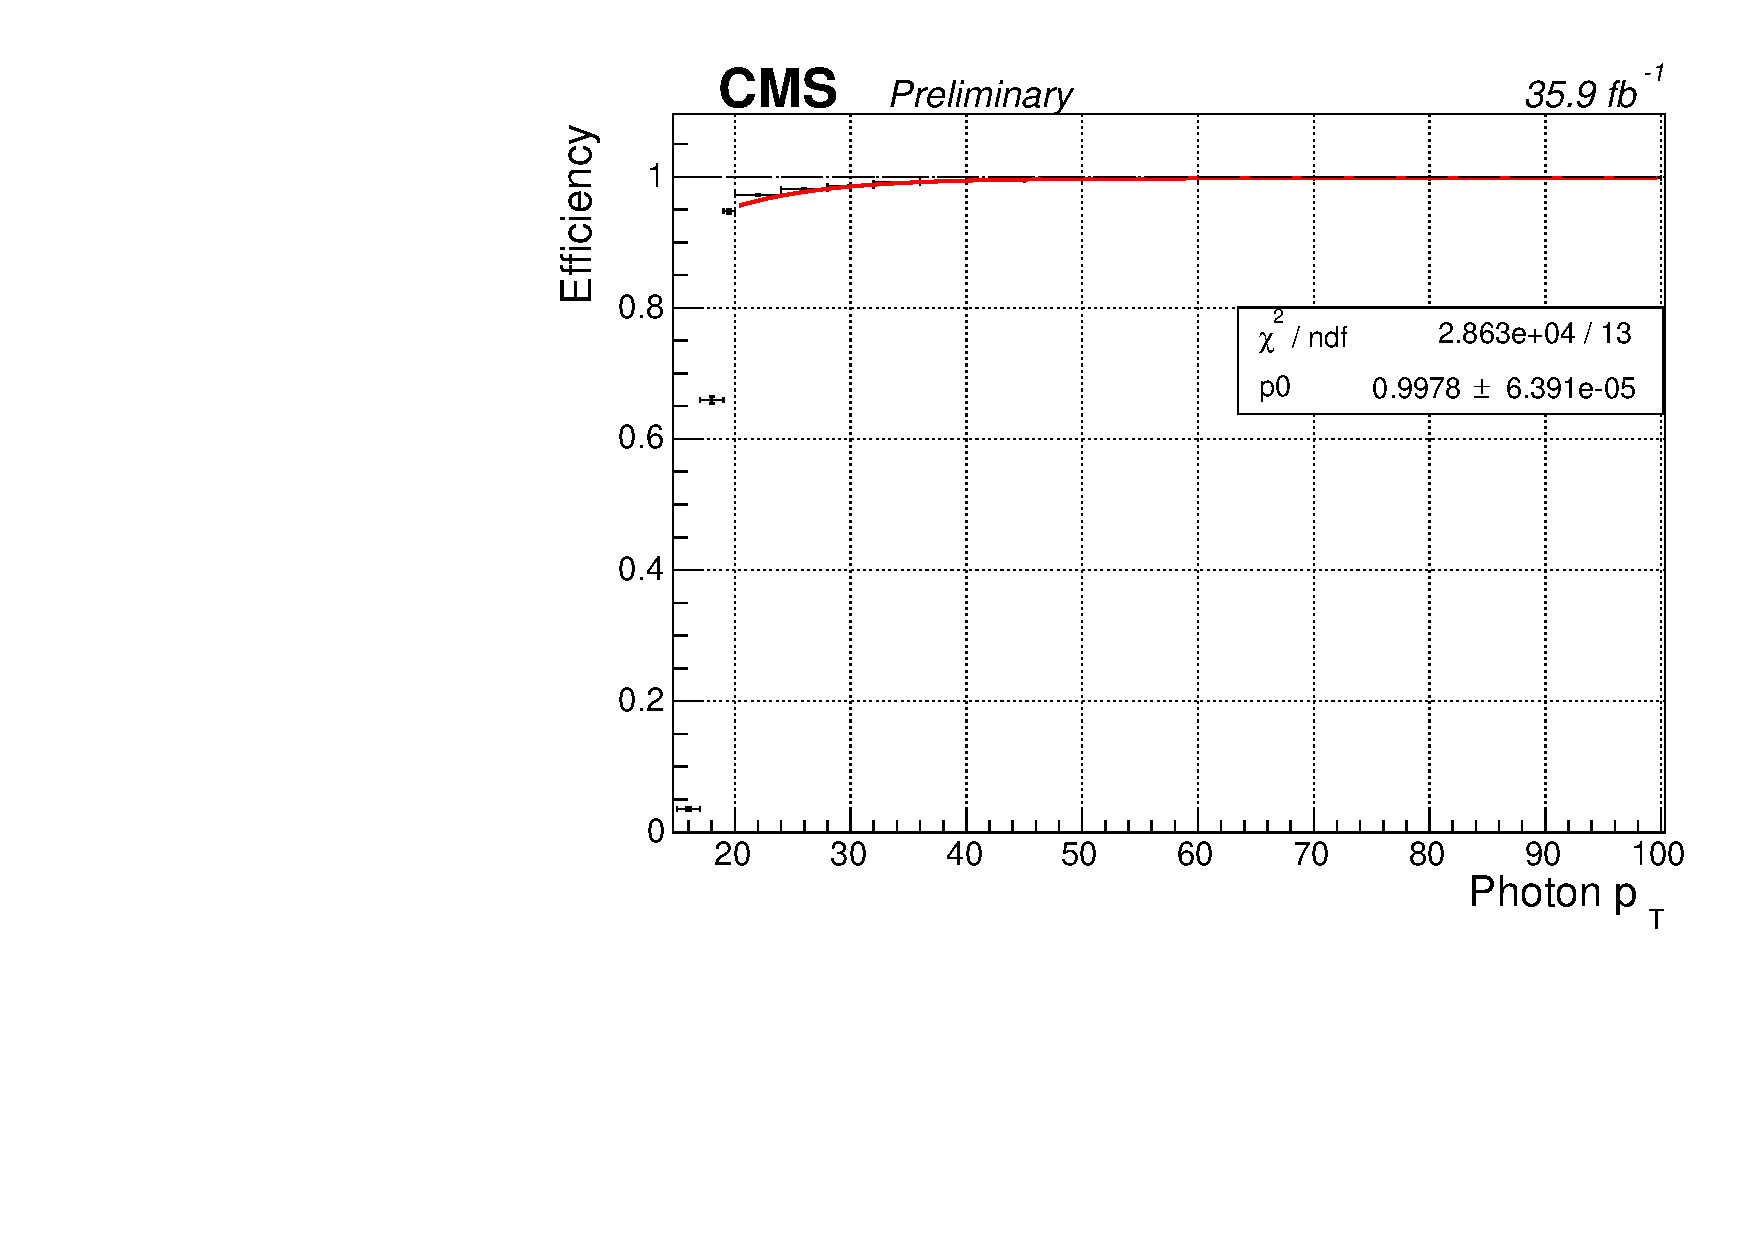
\includegraphics[width=0.9\textwidth]{Figures/Trigger/trailingEff.pdf}
\end{center}
\caption{Efficiency of the trailing leg of the primary analysis trigger with respect to photon \pT. 
For $\pT > 40$ GeV, the trigger is 99.8\% efficient.}
\label{fig:trailEff}
\end{figure*}

Finally, we calculated the efficiency of the trigger with respect to the diphoton invariant mass. For this calculation, we required two photons passing our analysis selection criteria, two photons satisfying the trailing leg of the trigger, and one photon passing the leading leg of the trigger. The efficiency was given by the number of diphoton events passing the full HLT path over the total number of diphoton events passing our requirements. The efficiency of the trigger as a function of invariant mass is shown in Figure~\ref{fig:InvMassEff}. For $m_{\gamma\gamma} > 100$ GeV, the trigger is 99.4\% efficient.

The efficiency of the trigger as a whole is the product of all three efficiencies. Two factors of the trailing leg efficiency are needed since both photons are required to pass that leg:
\begin{equation}
 \epsilon_{trig} = \epsilon_{lead} \times \epsilon_{trail}^2 \times \epsilon_{mass} = 97.2\%
\end{equation}

\begin{figure*}[h]
\begin{center}
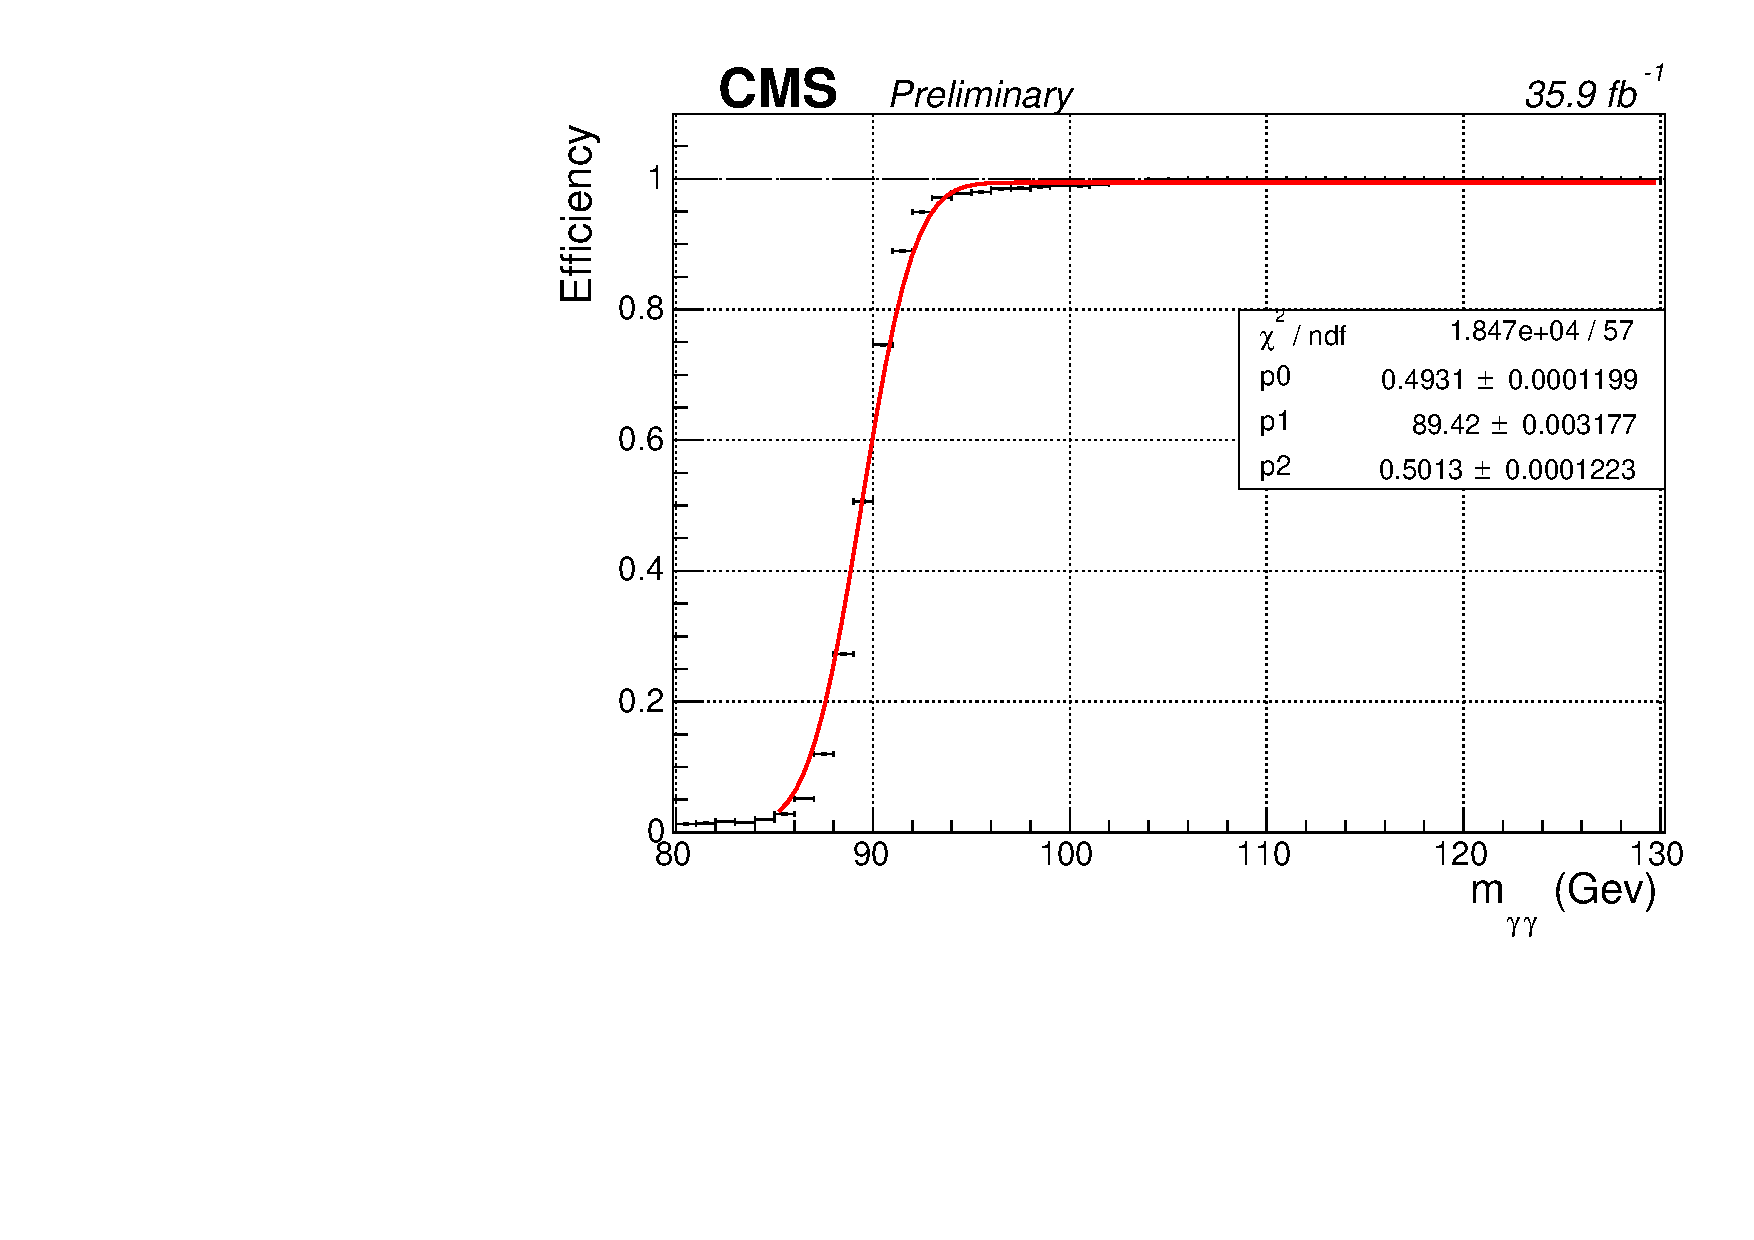
\includegraphics[width=0.9\textwidth]{Figures/Trigger/InvMassEff.pdf}
\end{center}
\caption{Efficiency of the primary analysis trigger with respect to the invariant mass of the diphoton system. 
For $m_{\gamma\gamma} > 100$ GeV, the trigger is 99.4\% efficient.}
\label{fig:InvMassEff}
\end{figure*}

\subsection{Efficiency of double electron trigger}
\label{sec:eeEff}
In the secondary trigger listed in Table~\ref{tab:triggers}, the pixel seed requirement is applied only to the trailing
leg of the trigger. This additional requirement results in a significantly lower overall efficiency for this leg. As shown in Figure~\ref{fig:controlTrailEff},
the trigger is only 90.4\% efficient for $\pT > 40$ GeV.
Since all other cuts are the same between the two triggers, however, the leading leg efficiency is the same as that shown in Figure~\ref{fig:leadEff}.
This results in an overall trigger efficiency of 79.8\% for the control trigger.

\begin{figure*}[h]
\begin{center}
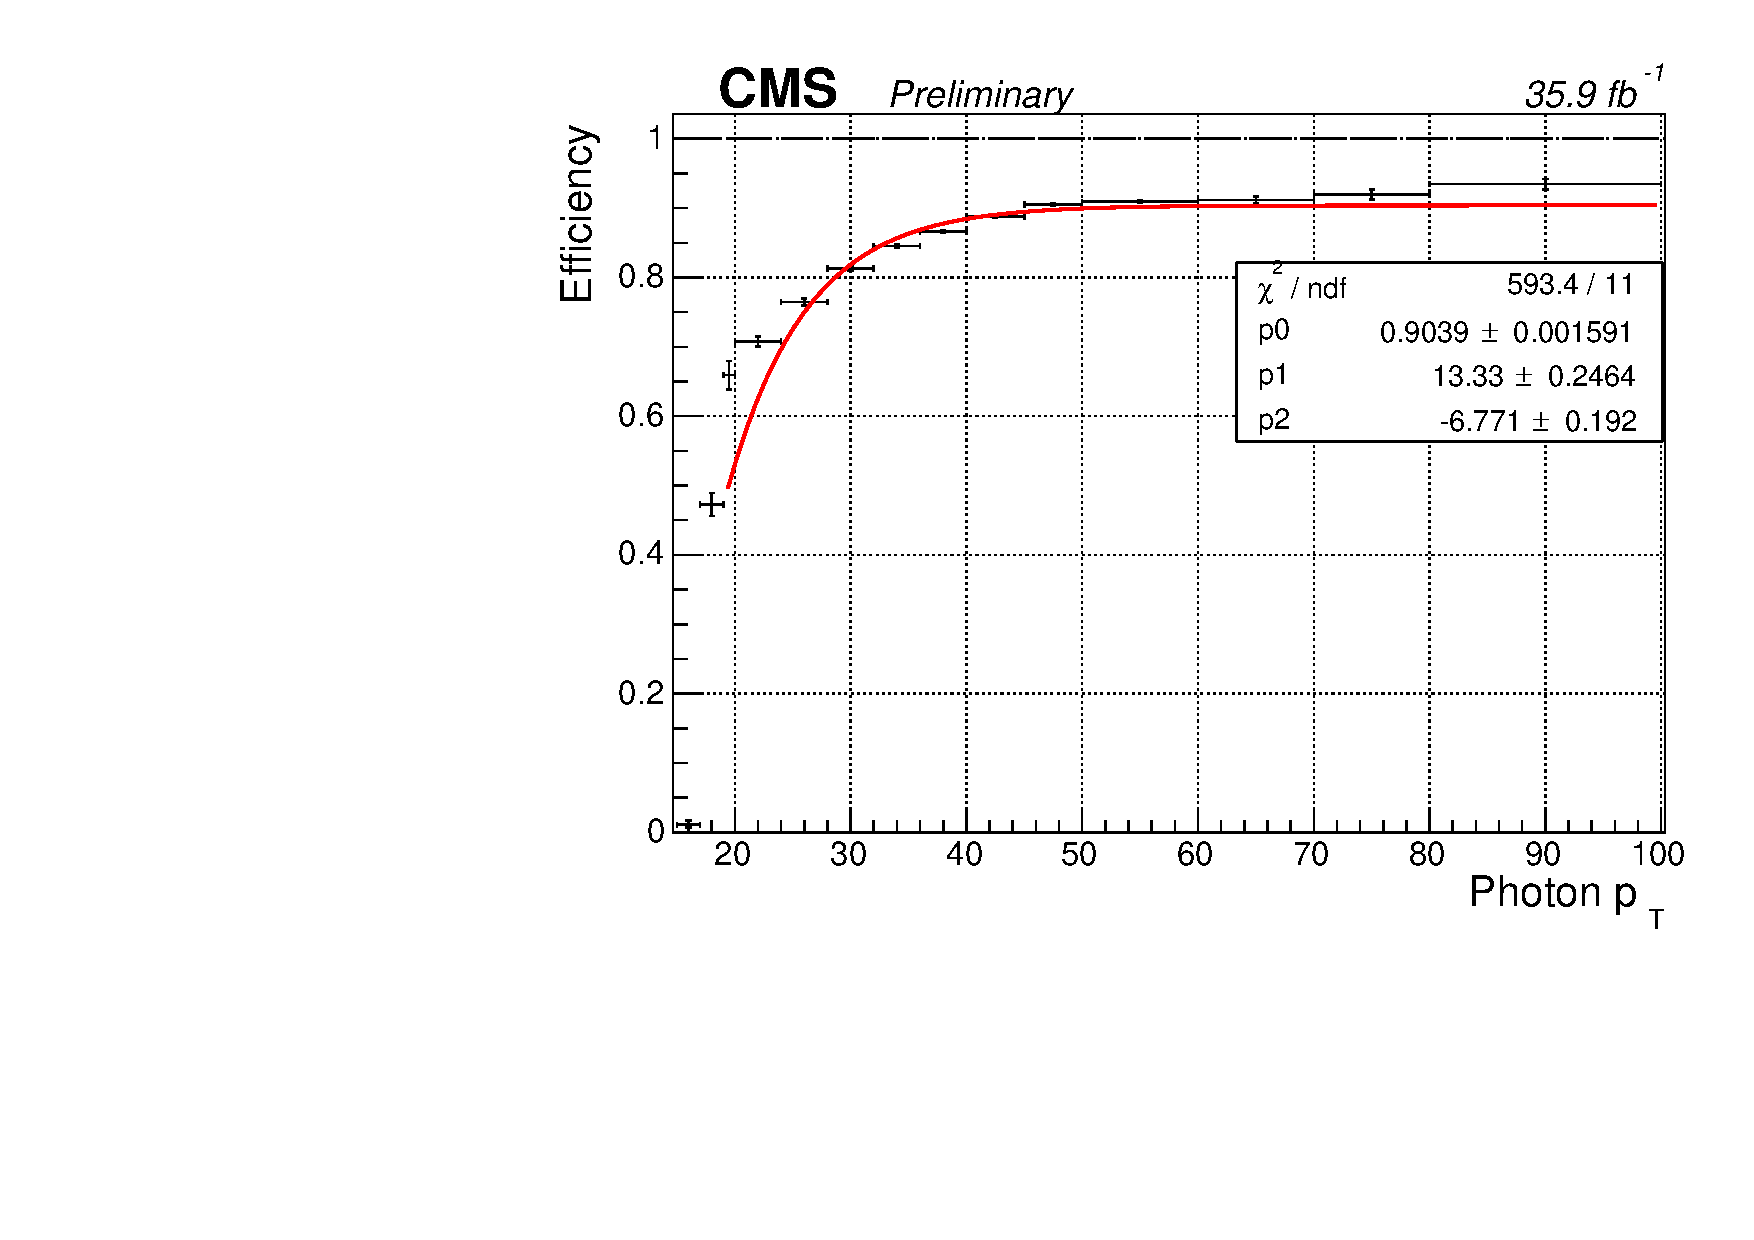
\includegraphics[width=0.9\textwidth]{Figures/Trigger/controlTrailingEff.pdf}
\end{center}
\caption{Efficiency of the trailing leg of the control trigger with respect to photon \pT. 
For $\pT > 40$ GeV, the trigger is 90.4\% efficient. The drop in efficiency with respect to the primary analysis 
trigger is caused by requiring both electromagnetic objects to be matched to a pixel seed.}
\label{fig:controlTrailEff}
\end{figure*}

